\documentclass[runningheads]{llncs}
\usepackage{accv}
\usepackage{graphicx,booktabs}
% axessibility's pdfTeX-only primitives are incompatible with Tectonic/XeTeX.
\usepackage[breaklinks,colorlinks,citecolor=accvblue,urlcolor=black,linkcolor=black]{hyperref}
\hypersetup{pdftitle={The Delegation Blind Spot: Auditing Product Decisions from Agent Choices},pdfauthor={Shivam Gupta}}
\begin{document}
\title{The Delegation Blind Spot: Auditing Product Decisions from Agent Choices}
\titlerunning{The Delegation Blind Spot}
\author{Shivam Gupta}
\authorrunning{S. Gupta}
\institute{Independent Researcher, Dubai, United Arab Emirates\\\email{shivam1720406@gmail.com}}
\maketitle
\begin{abstract}
A successful agent action need not reveal which product improvement its user would value. We present a decision-specific audit mapping a declared observation channel and product comparison to compatible value intervals and witness populations. In 4,800 requests to two pinned models on synthetic tasks, all 36 conservative primary comparisons remain unresolved despite different execution accuracy. An exploratory 2,400-call follow-up records supplied preferences and resolves three of nine comparisons per model; a deterministic extractor resolves seven without model calls. Controlled simulations separate structural ambiguity from finite-sample uncertainty. The contribution is an executable measurement workflow using established identification principles, not a new general estimator. The study has no human participants or customer validation and does not evaluate multimodal models.
\keywords{AI agents \and measurement \and partial identification}
\end{abstract}

\section{What does a successful action tell the analyst?}
Two agents book the same hotel, one for quiet and one for proximity to a meeting. Both bookings can be optimal, while their transaction records cannot distinguish demand for soundproofing from demand for transport links. The analyst's future decision differs from the agent's current task. Human choices can share this ambiguity; delegation does not create a new impossibility theorem.

We ask whether a specified observation supports a specified product comparison. Delegated choice, preference transmission, and revealed-preference alignment have direct antecedents \cite{kops2026,kraft2026,suleymanov2026}. Rich menu variation can identify quantities that coarse transaction categories cannot. Our audit operationalizes established experiment comparison, label-shift estimation, and measurement-error partial identification \cite{blackwell1953,lipton2018,finkelstein2021}. Its relevance to measurement from incomplete observations is methodological: the experiments concern text-conditioned agent choices, not multimodal perception or physical-science discovery.

\section{A calibrated decision audit}
Let $p\geq0$, $\mathbf1^Tp=1$ be proportions of $K$ declared intent classes. A column-stochastic channel $A$ maps class to logged category, giving $q=Ap$. A separately specified class contrast $d_k$ represents the value difference between future product variants. The target is $\Delta=d^Tp$. For known $A,q$, the audit minimizes and maximizes this target over $\mathcal P_q=\{p\geq0:\mathbf1^Tp=1,Ap=q\}$. A strictly positive lower bound or negative upper bound resolves the comparison; otherwise it abstains and returns the endpoint mixtures as witnesses. Witnesses are compatible populations, not estimates of real individuals.

For known $A$, $d^Tp$ is identified for every feasible $q$ exactly when $d$ belongs to the row space of $A$. If $d=A^Tv$, then $d^Tp=v^Tq$. Otherwise a null-space direction changes the target without changing the log. This standard structural result does not imply that finite samples yield useful precision.

For uncertain $A,q$, introduce joint masses $J_{ak}=A_{ak}p_k$ and solve the linear program with constraints
\begin{equation}
\begin{split}
p\geq0,\quad \mathbf1^Tp=1,\quad J\geq0,\quad \sum_aJ_{ak}=p_k,\\
\underline A_{ak}p_k\leq J_{ak}\leq\overline A_{ak}p_k,\quad
\underline q_a\leq\sum_kJ_{ak}\leq\overline q_a.
\end{split}
\end{equation}
Minimizing and maximizing $d^Tp$ gives attainable bounds within these rectangular restrictions. Simultaneous coordinate Clopper--Pearson bounds allocate errors .02 to calibration and .02 to field frequencies. The resulting coverage is at least 96\% marginally per predeclared comparison, assuming independent sampling, stable channels, correct classes, and known $d$. It is not simultaneous coverage over every reported comparison. Infeasibility is a diagnostic failure, not a resolved decision.

\section{Computational evidence}
\paragraph{Frozen primary design.}
GPT-5.4 Mini and Nano, pinned to their 17 March 2026 snapshots, each receive the same 2,400 tasks. Travel, cloud plans, and workflow software are three framings of one generator. Four synthetic profiles supply numerical attribute weights and a minimum-attribute penalty. Menus contain four perturbed alternatives in randomized order. Per model and framing, calibration uses 80 tasks per class; three field mixtures each use 160 tasks. Calibration classes are known by construction and are withheld from the field estimator.

The future comparison is capacity versus flexibility investment with the same affordability tradeoff. Class contrasts are exact means over an independent 4,096-menu bank, assuming optimal future selection rather than measuring future model behavior. Logs retain product type or type plus context, including failure categories, but omit the full continuous menu. This isolates a synthetic measurement problem; real product value would require independent outcome evidence.

Of 4,800 attempts, 4,783 yield valid choices and 17 retain transport failures without replacement retries. Mini selects a utility maximizer in 73.19\% of field tasks; Nano does so in 55.69\%. All 18 comparisons per model remain unresolved, including those for an optimal-choice control. This does not establish structural nonidentification. Shared data across comparisons also prevent interpreting the observed target-containment fraction as an empirical coverage estimate.

\paragraph{Exploratory information control.}
A subsequent frozen follow-up asks for the largest weight already supplied in the profile. It uses 40 calibration tasks per class and 80 field tasks per mixture and framing, selected by task ID independently of response correctness. Each model makes 1,200 new calls, repeating only 12 distinct prompts. Every report is correct. The leading attribute uniquely identifies the constructed class, so this is extraction of known input, not learning a person's preferences. Both models resolve 3/9 comparisons versus 0/9 for matched action-only logs (Table~\ref{tab:results}). Observation counts are matched, not cost, privacy exposure, or elicitation burden. The data-motivated follow-up has no selective-inference correction.

\begin{table}[t]
\caption{Paired results, with 80 field tasks per condition. The deterministic parser uses a known identity channel; model reports estimate that channel.}
\label{tab:results}
\centering
\begin{tabular}{lrrr}
\toprule Observation & Mini & Nano & Mean width \\
\midrule
Action only & 0/9 & 0/9 & 0.08720 \\
Supplied-weight report & 3/9 & 3/9 & 0.04360 \\
Deterministic parser & \multicolumn{2}{c}{7/9, shared tasks} & 0.02285 \\
\bottomrule
\end{tabular}
\end{table}

\paragraph{Separate information from precision.}
For $A_\eta=(1-\eta)\mathbf1\mathbf1^T/4+\eta I_4$, all classes have the same log at $\eta=0$; the channel is full rank at every $\eta>0$. Across six strengths, four calibration budgets and three mixtures, 200 repetitions per cell generate 14,400 multinomial datasets. At $\eta=.01$, even 2,560 calibration observations per class and 5,120 field observations leave all joint intervals unresolved. Known-channel, known-frequency and joint ablations have 98\%, 98\% and 96\% marginal guarantees and are not an equal-confidence ranking.

A deterministic supplied-weight parser instead uses a known identity channel on the same 720 field records. At 96\% marginal coverage it resolves 7/9 comparisons, with no incorrect resolutions, calibration observations or API calls. Separate direct Hoeffding intervals also resolve 7/9; they are not intersected with the first intervals. These controls expose avoidable report-channel calibration uncertainty.

\section{Implications, limits and provenance}
\begin{figure}[t]
\centering
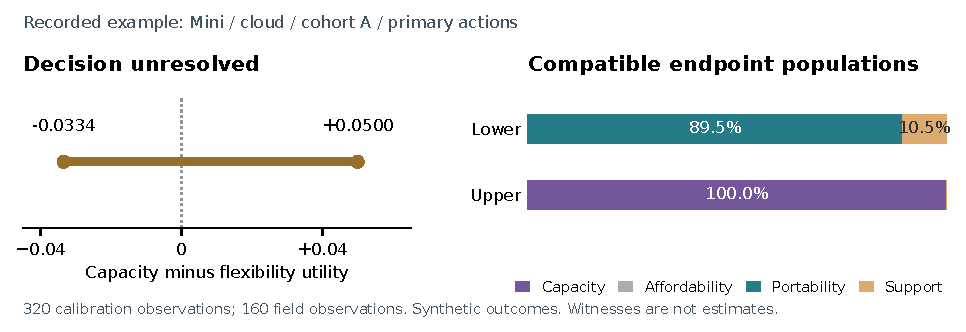
\includegraphics[width=\linewidth]{../../generated/audit-example.pdf}
\caption{One recorded inspector condition. The contrast interval crosses zero, from $-0.0334$ to $0.0500$. Its endpoint witnesses are different synthetic populations compatible with the same uncertainty restrictions, not inferred customer segments. They need not share one exact channel.}
\label{fig:audit}
\end{figure}
The offline diagnostic viewer displays recorded intervals, endpoint witnesses, contrast definitions and counts. A proposed decision receipt distinguishes observed actions, supplied constraints, inferred explanations and independently confirmed outcomes. It should preserve consent and measurement conditions rather than promote an agent's explanation into customer evidence. An unresolved interval calls for diagnosing the information gap before collecting more of the same telemetry. Usability, business outcomes and the complete receipt interface remain untested.

The study contains no human participants or customer validation. It covers one synthetic task family and two related model snapshots. Unknown classes, drift, dependence and incorrect utility contrasts can invalidate the audit. Preserving a supplied profile does not validate it against the person represented.

\paragraph{AI assistance.}
OpenAI Codex assisted with formulation, literature retrieval, proof drafting, experiment design, code, analysis, figures and writing. Internal AI critiques are not independent peer review. Primary-source checks, counterexamples, numerical witnesses, tests, frozen response records and exact reanalysis support verification but do not replace human-author scrutiny and accountability.

\paragraph{Disclosure and artifacts.}
A substantially overlapping short version is under review at IUI 2027 Posters, submission 5609; no acceptance is claimed. This version is submitted solely for non-archival workshop presentation. Code, full proofs, frozen designs, model records and the viewer accompany the technical report at \url{https://github.com/shi1720/delegation-blind-spot}.

\bibliographystyle{splncs04}
\bibliography{../../references}
\end{document}
